\subsection{Lax-Wendroff Scheme}

Ideally, a second order numerical scheme has the form
$\tilde{u}_{j,k+1}={\color{orange}A}\cdot\tilde{u}_{i+1,k}+{\color{red}B}\cdot\tilde{u}_{i,k}+{\color{blue}C}\cdot\tilde{u}_{j-1,k}$.
Concretely, for the advection equation, the coefficients would be
\begin{align*}
	{\color{orange} A={\frac{r^{2}-r}{2}}},\;\;{\color{red} B=1-r^{2}},\;\;
	{\color{blue} C={\frac{r^{2}+r}{2}}}\quad
	{\color{gray} (r = \frac{\Delta t}{\Delta x})}
\end{align*}

\makebox[\columnwidth]{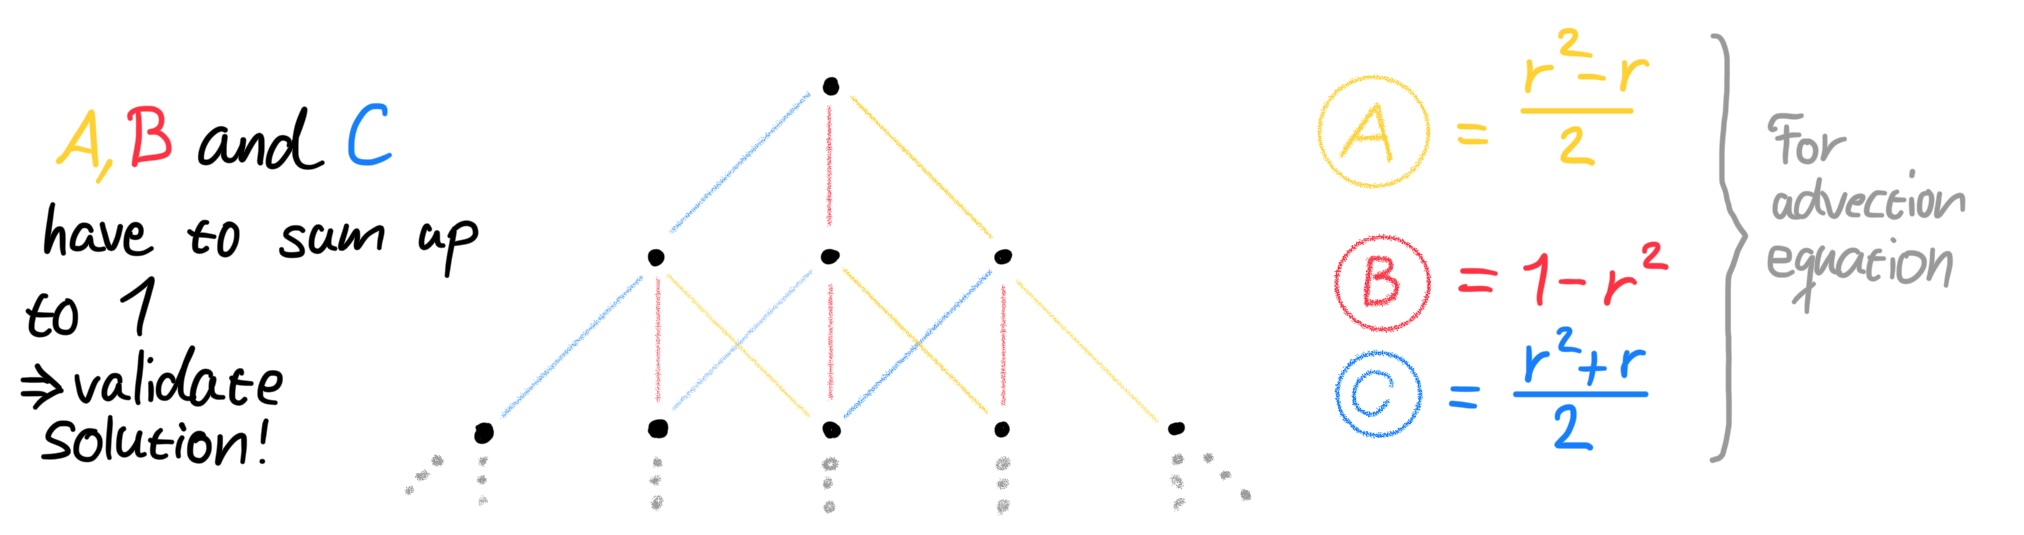
\includegraphics[width=0.8\columnwidth]{images/lax_wendroff_scheme}}